\documentclass[10pt,letterpaper]{article}
\usepackage[utf8]{inputenc}
\usepackage{amsmath}
\usepackage{amsfonts}
\usepackage{amssymb}
\usepackage{graphicx}
\usepackage[left=2cm,right=2cm,top=2cm,bottom=2cm]{geometry}
\author{Joey Harrington}
\title{SteadyHand}
\begin{document}
\maketitle
\section*{The Experiment}
For this experiment we collected data of individuals attempting to hold a laser steady. With the help of a MotionLogger, we were able to track the movement of the laser. The MotionLogger has the ability to track and log the position of objects in a video. The individuals took turns holding the laser at a fixed point at two distances. Each student held the laser at a distance of 5 meters for approximately 15 seconds and again at a distance of 10 meters for the same amount of time. The data was collected and made into text files. From there we were able to construct scripts that processed the data to determine who had the steadiest hand.
\section*{Results}
\begin{center}
\begin{table}[h!]
\centering
\begin{tabular}{|c|c|c|c|c|c|} 
 \hline
 Filename & x-avg & y-avg & x-dev & y-dev & total-dev \\ 
 \hline\hline
 \input{1-ranking-short.txt}
 \hline
\end{tabular}
\caption{Table of the rankings from the short distance for one second.}
\label{table:1}
\end{table}
\end{center}
\begin{center}
\begin{table}[h!]
\centering
\begin{tabular}{|c|c|c|c|c|c|} 
 \hline
 Filename & x-avg & y-avg & x-dev & y-dev & total-dev \\ 
 \hline\hline
 \input{1-ranking-long.txt}
 \hline
\end{tabular}
\caption{Table of the rankings from the long distance for one second.}
\label{table:2}
\end{table}
\end{center}
\begin{center}
\begin{table}[h!]
\centering
\begin{tabular}{|c|c|c|c|c|c|} 
 \hline
 Filename & x-avg & y-avg & x-dev & y-dev & total-dev \\ 
 \hline\hline
 \input{10-ranking-short.txt}
 \hline
\end{tabular}
\caption{Table of the rankings from the short distance for ten seconds.}
\label{table:3}
\end{table}
\end{center}
\begin{center}
\begin{table}[h!]
\centering
\begin{tabular}{|c|c|c|c|c|c|} 
 \hline
 Filename & x-avg & y-avg & x-dev & y-dev & total-dev \\ 
 \hline\hline
 \input{10-ranking-long.txt}
 \hline
\end{tabular}
\caption{Table of the rankings from the long distance for ten seconds.}
\label{table:4}
\end{table}
\end{center}
\clearpage
\section*{Histogram}
\paragraph*{} We were able to create a script that calculated the distance from each points position to the average position for each file. We then generated a histogram that used the first ten seconds of all data files. Our histogram shows the count for these distances. 
\begin{figure}
\caption{A graph that shows the count for the distance from average for each data file.}
\graphicspath{ {./} }
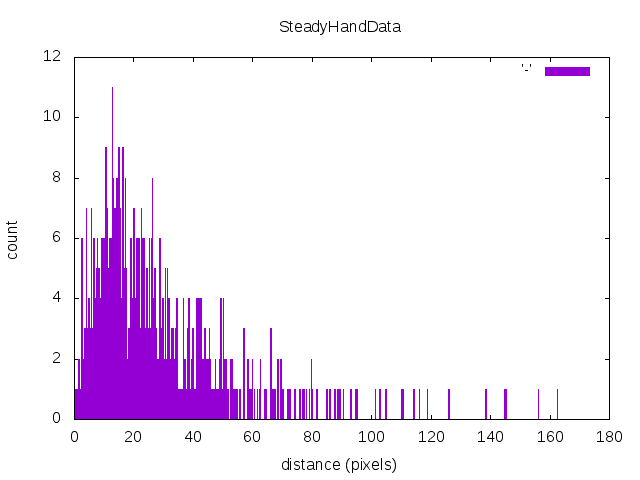
\includegraphics{histogram}
\end{figure}
\end{document}